%!TEX root = ../../main.tex

\chapter{Image Representation}

\section{Appearance}
\label{sec:appearance}
In the \giraf software-suite there exist various types of images, such as pictograms and profile pictures. Images should be quadratic, have a white background regardless of content and have a black border, as seen on Figure \ref{fig:pictogram_image_view}. 

\todo{Refer to black}

\begin{figure}[!htbp]
    \centering

    \begin{subfigure}[t]{0.4\textwidth}
    	\centering
        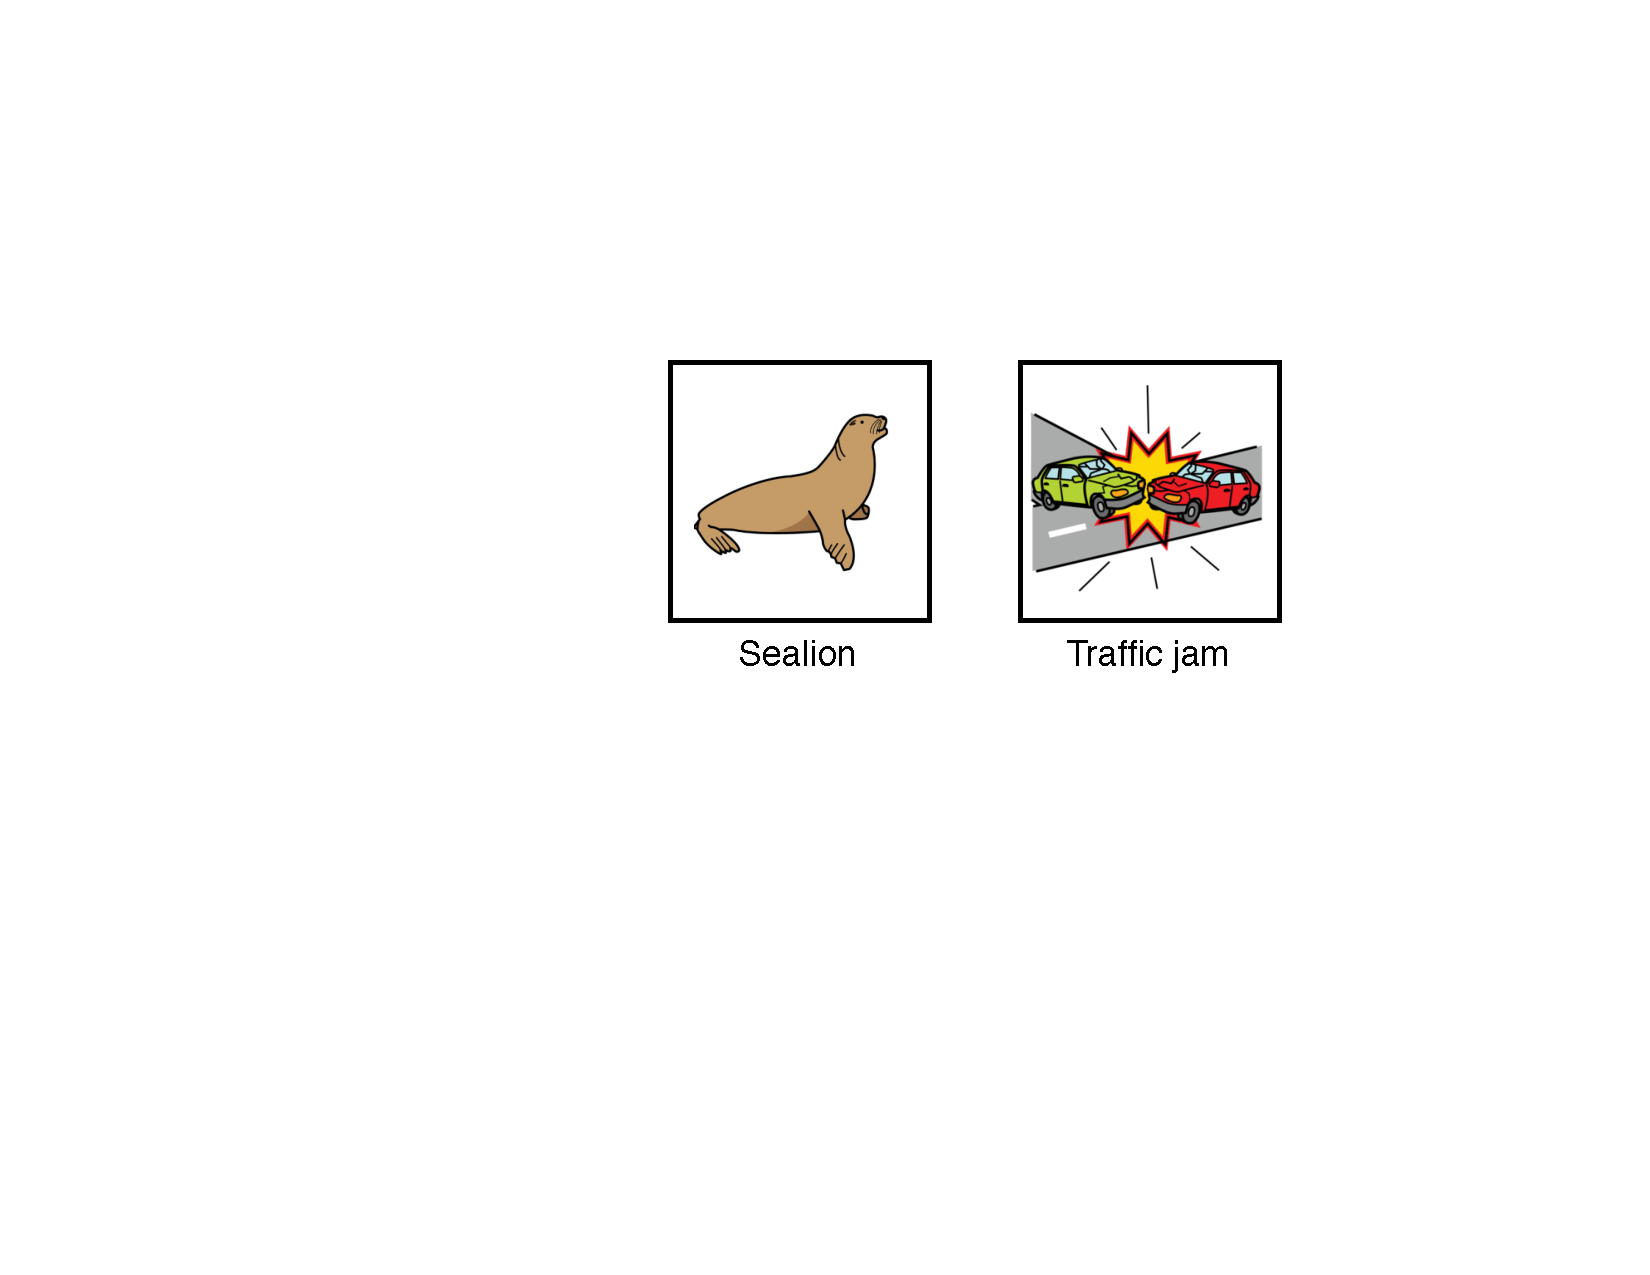
\includegraphics[scale=0.5]{pictogram_image_view_pictograms}
        \caption{Pictograms}
        \label{fig:pictogram_image_view_pictograms}
    \end{subfigure}
    \hspace{5em} 
    \begin{subfigure}[t]{0.4\textwidth}
    	\centering
        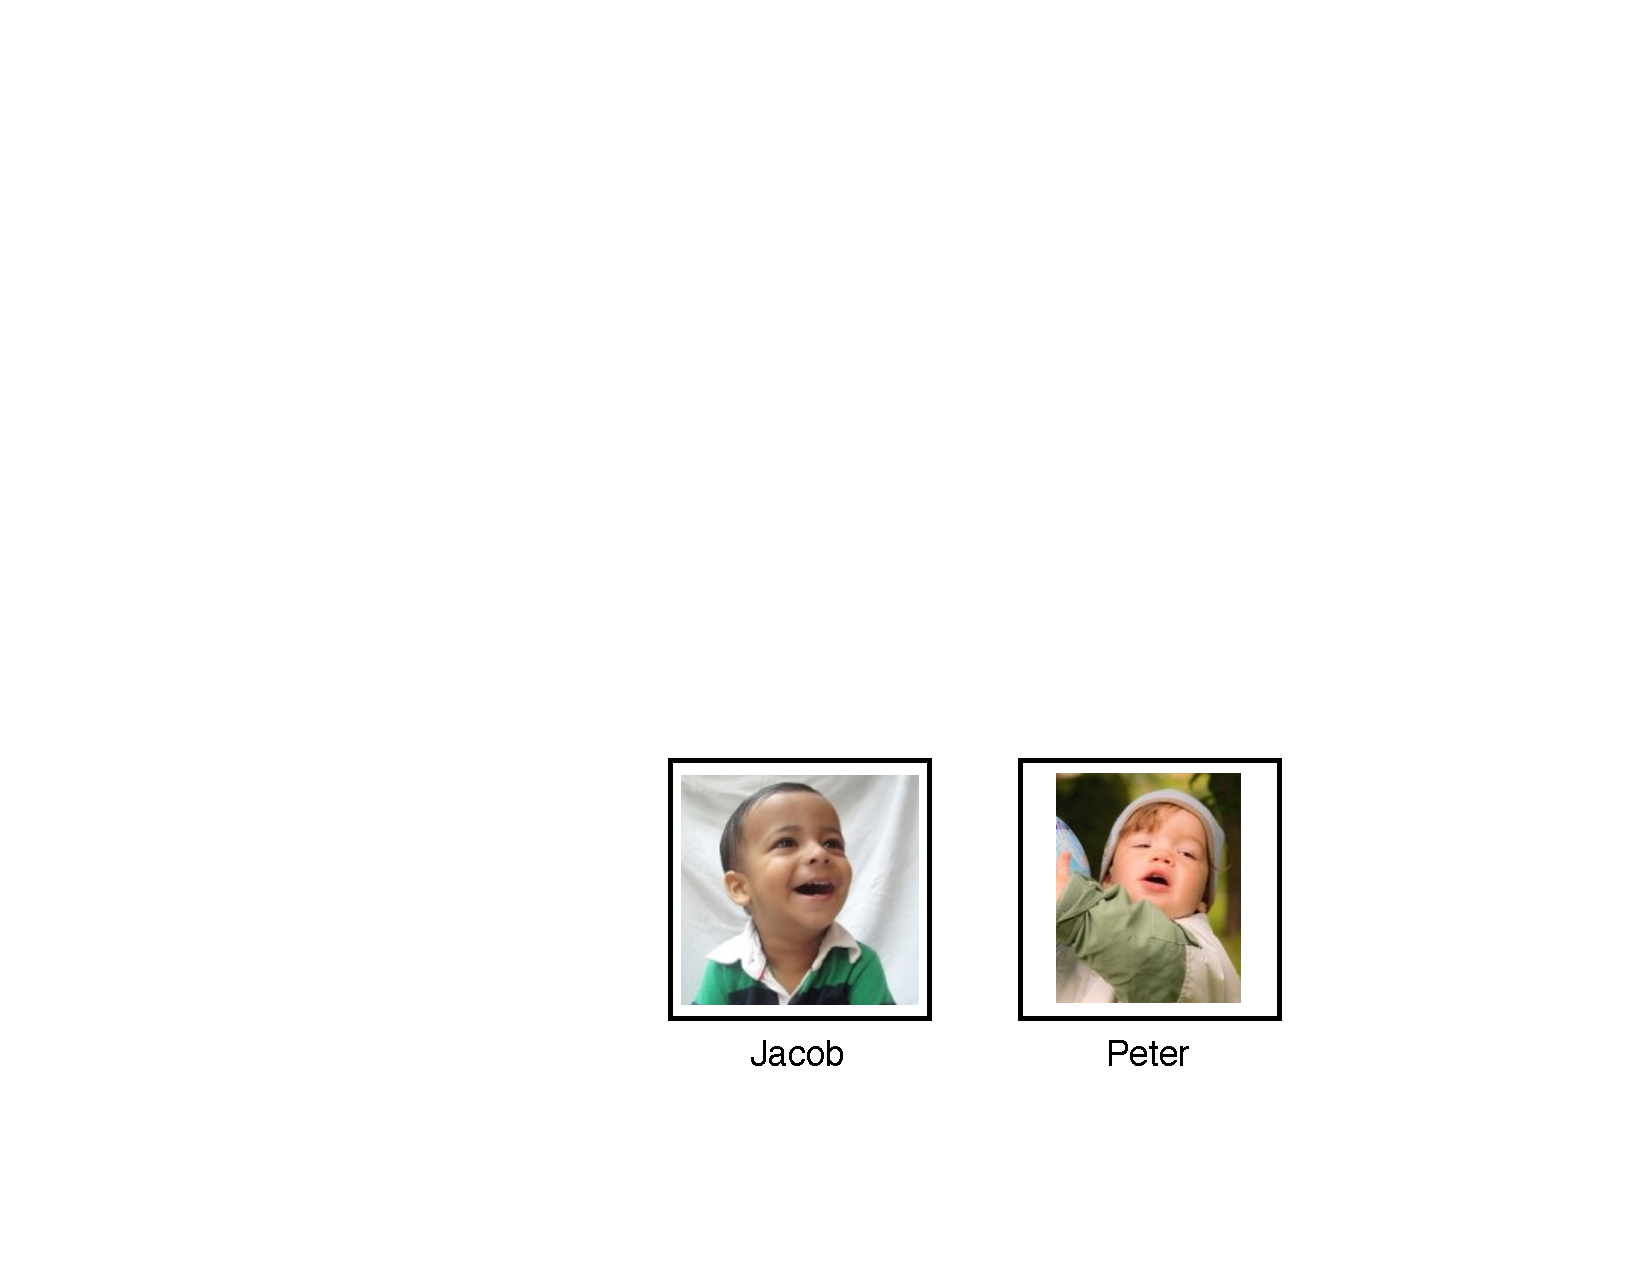
\includegraphics[scale=0.5]{pictogram_image_view_profiles}
        \caption{Profile pictures}
        \label{fig:pictogram_image_view_profiles}
    \end{subfigure}
    
    \caption{Image representation}
    \label{fig:pictogram_image_view}
\end{figure}

\begin{note}
	Profile pictures as seen on Figure \ref{fig:pictogram_image_view_profiles} should, as the first profile (Jacob), fit to the canvas. How ever many profile pictures are captured in a different way as the second profile (Peter). It is wanted that in the future when profile picuters are captured that the allow for the layout of the first profile. But for the sake of convinience we allow old profile pictures toe be as the second.
\end{note}

\noindent
The image view shoud have a 10 dp padding so that the content gets spacing to the border as seen on Figure \ref{fig:pictograms_padding}.

\begin{figure}[h]
	\centering
	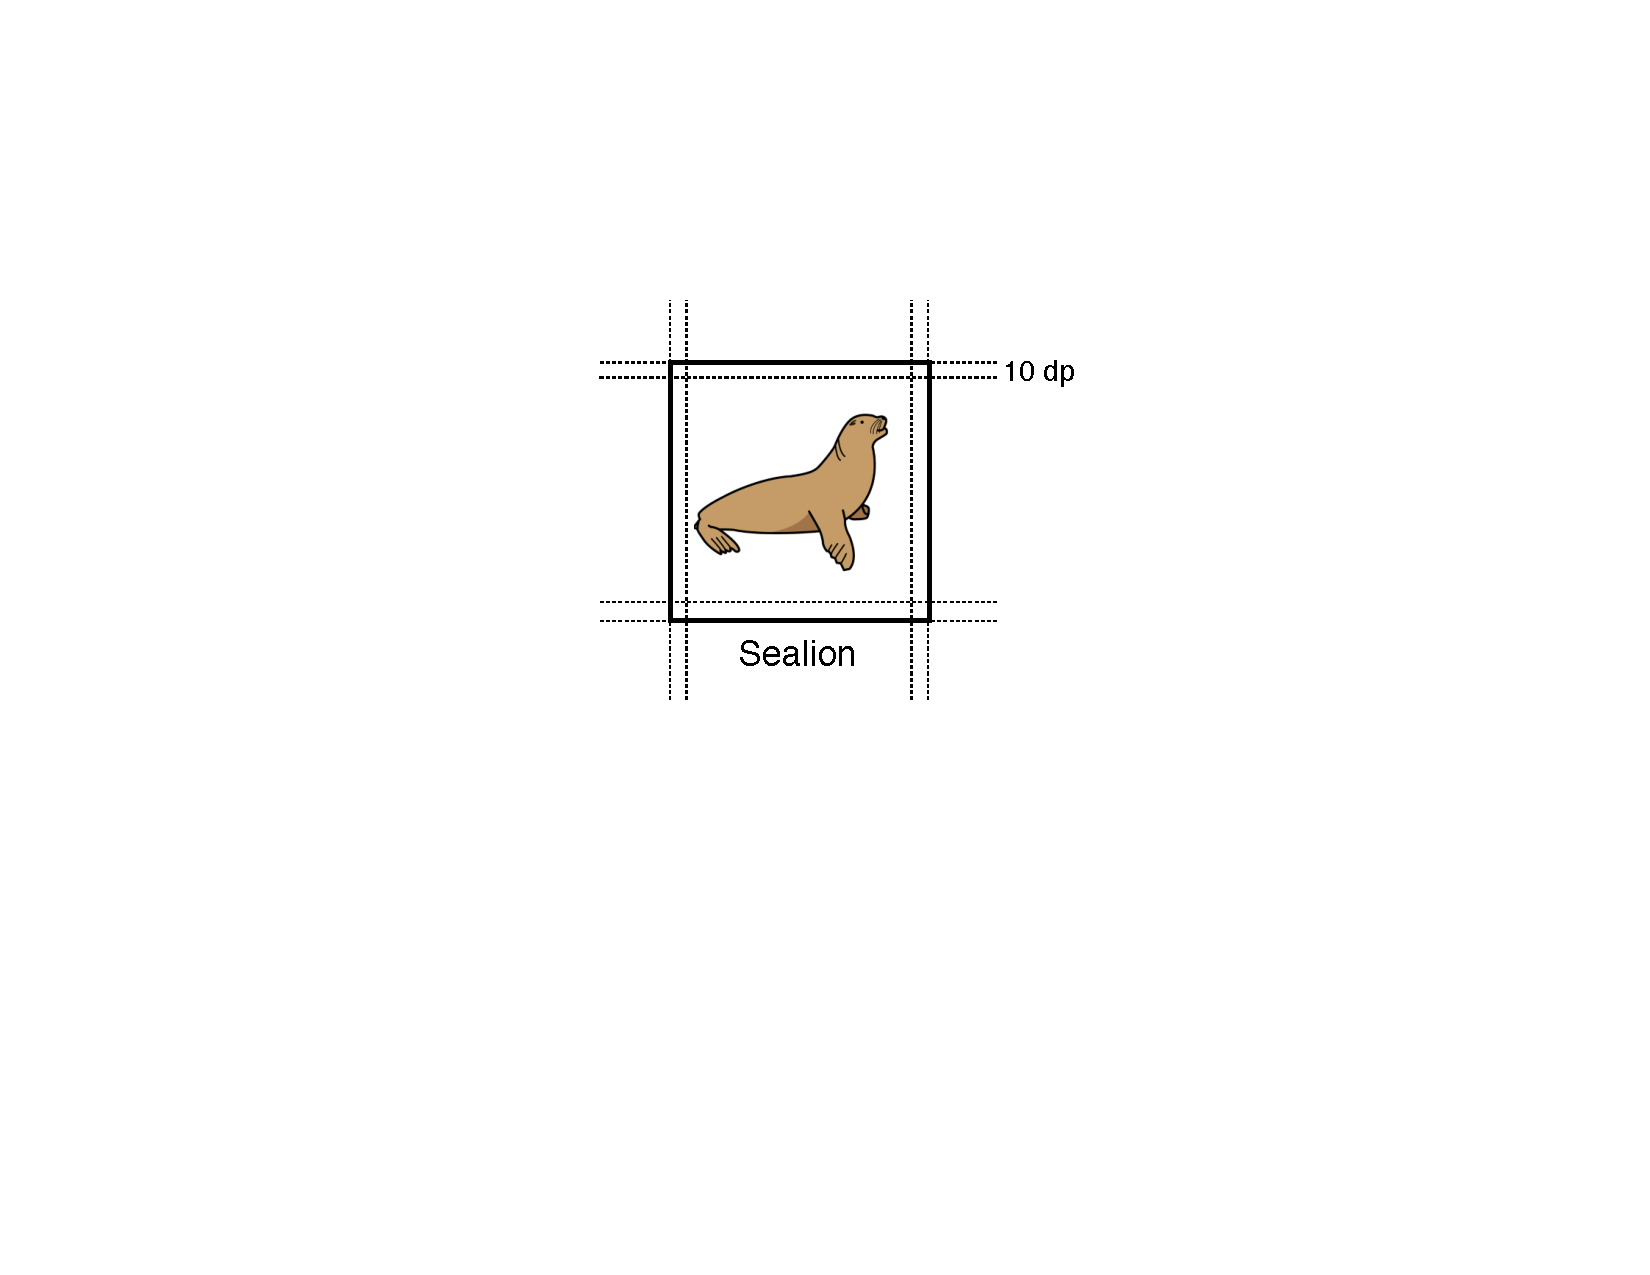
\includegraphics[width=0.35\textwidth]{pictograms_padding}
	\caption{Image representation}
	\label{fig:pictograms_padding}
\end{figure} 
\FloatBarrier

\section{Marking}
\label{sec:marking}
It is often possible to mark images, in this case one should mark the background with an orange color \todo{refer to organge color}, as seen on Figure \ref{fig:pictograms_marked}. 

\begin{figure}[!htbp]
    \centering

    \begin{subfigure}[t]{0.4\textwidth}
    	\centering
        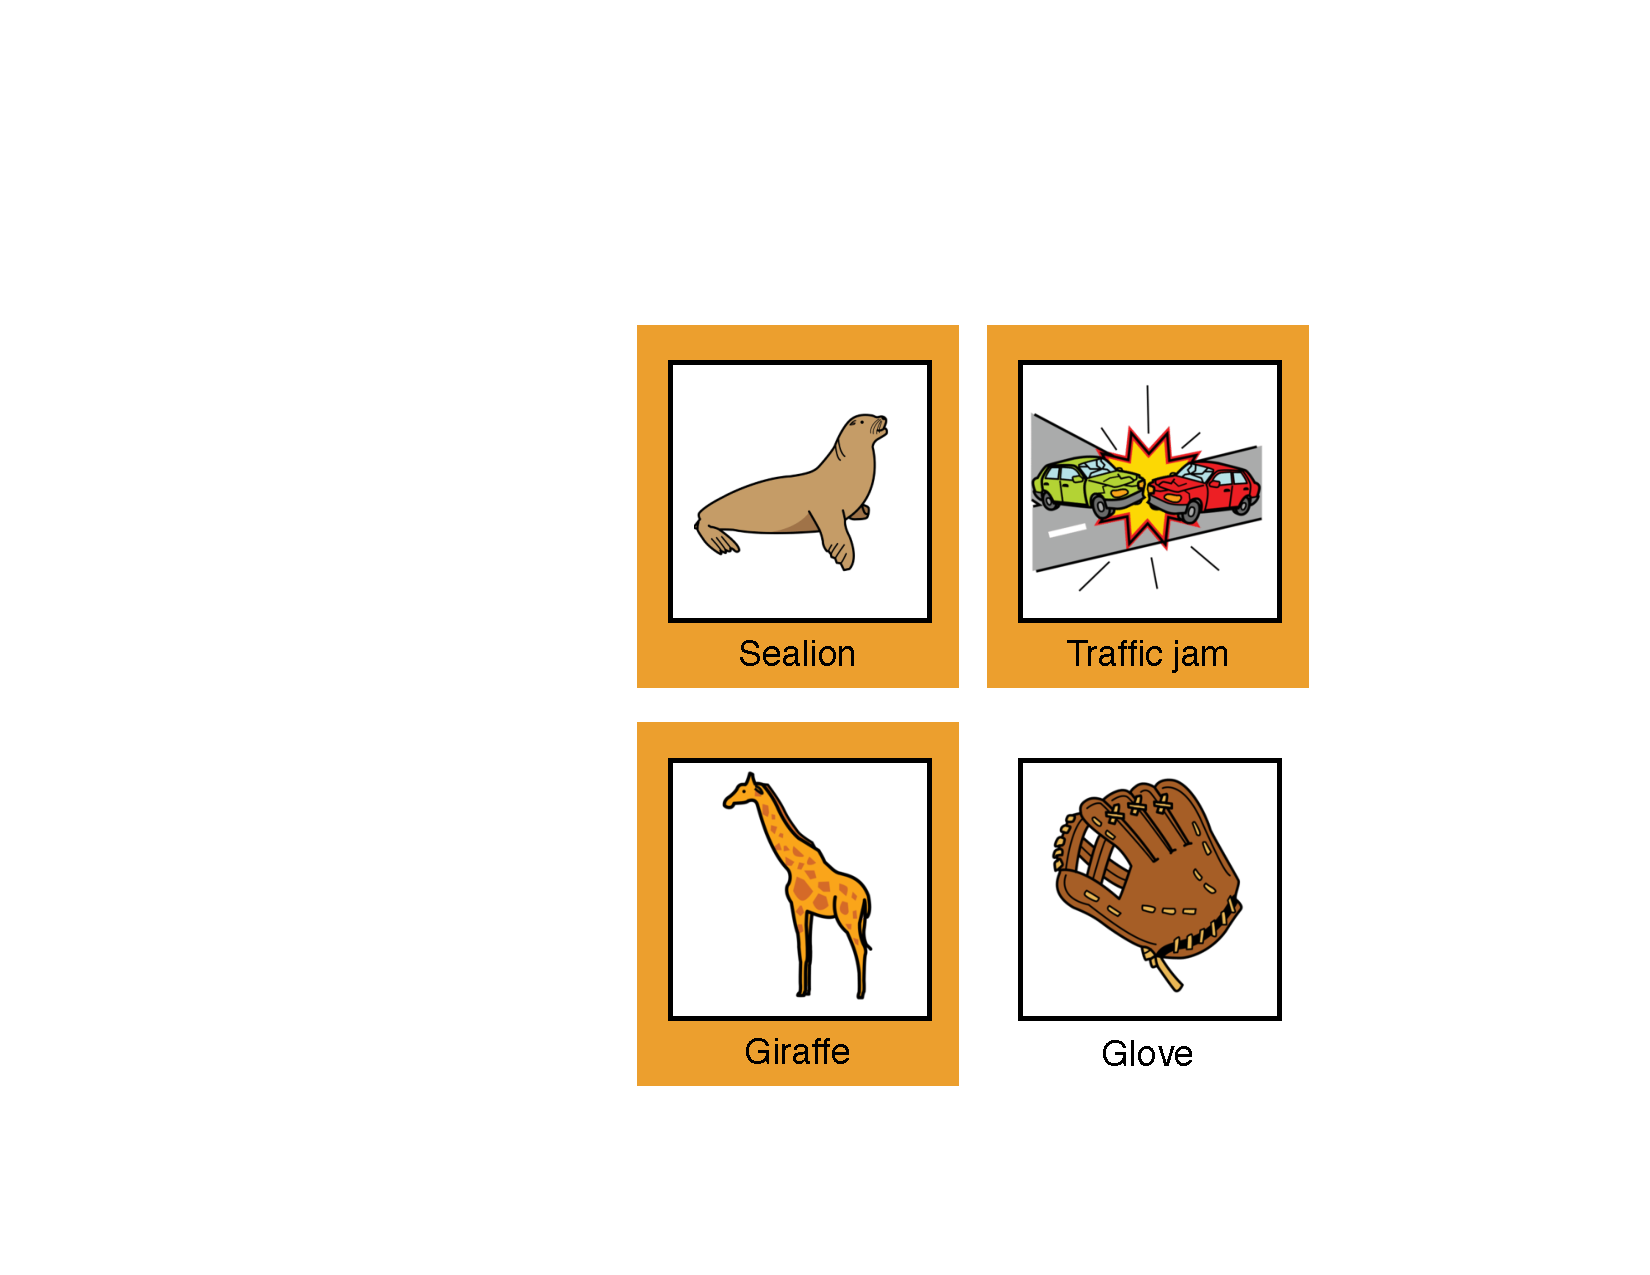
\includegraphics[scale=0.5]{pictograms_marked_correct}
        \caption{Corrected marking}
        \label{fig:pictograms_marked_corect}
    \end{subfigure}
    \hspace{5em} 
    \begin{subfigure}[t]{0.4\textwidth}
    	\centering
        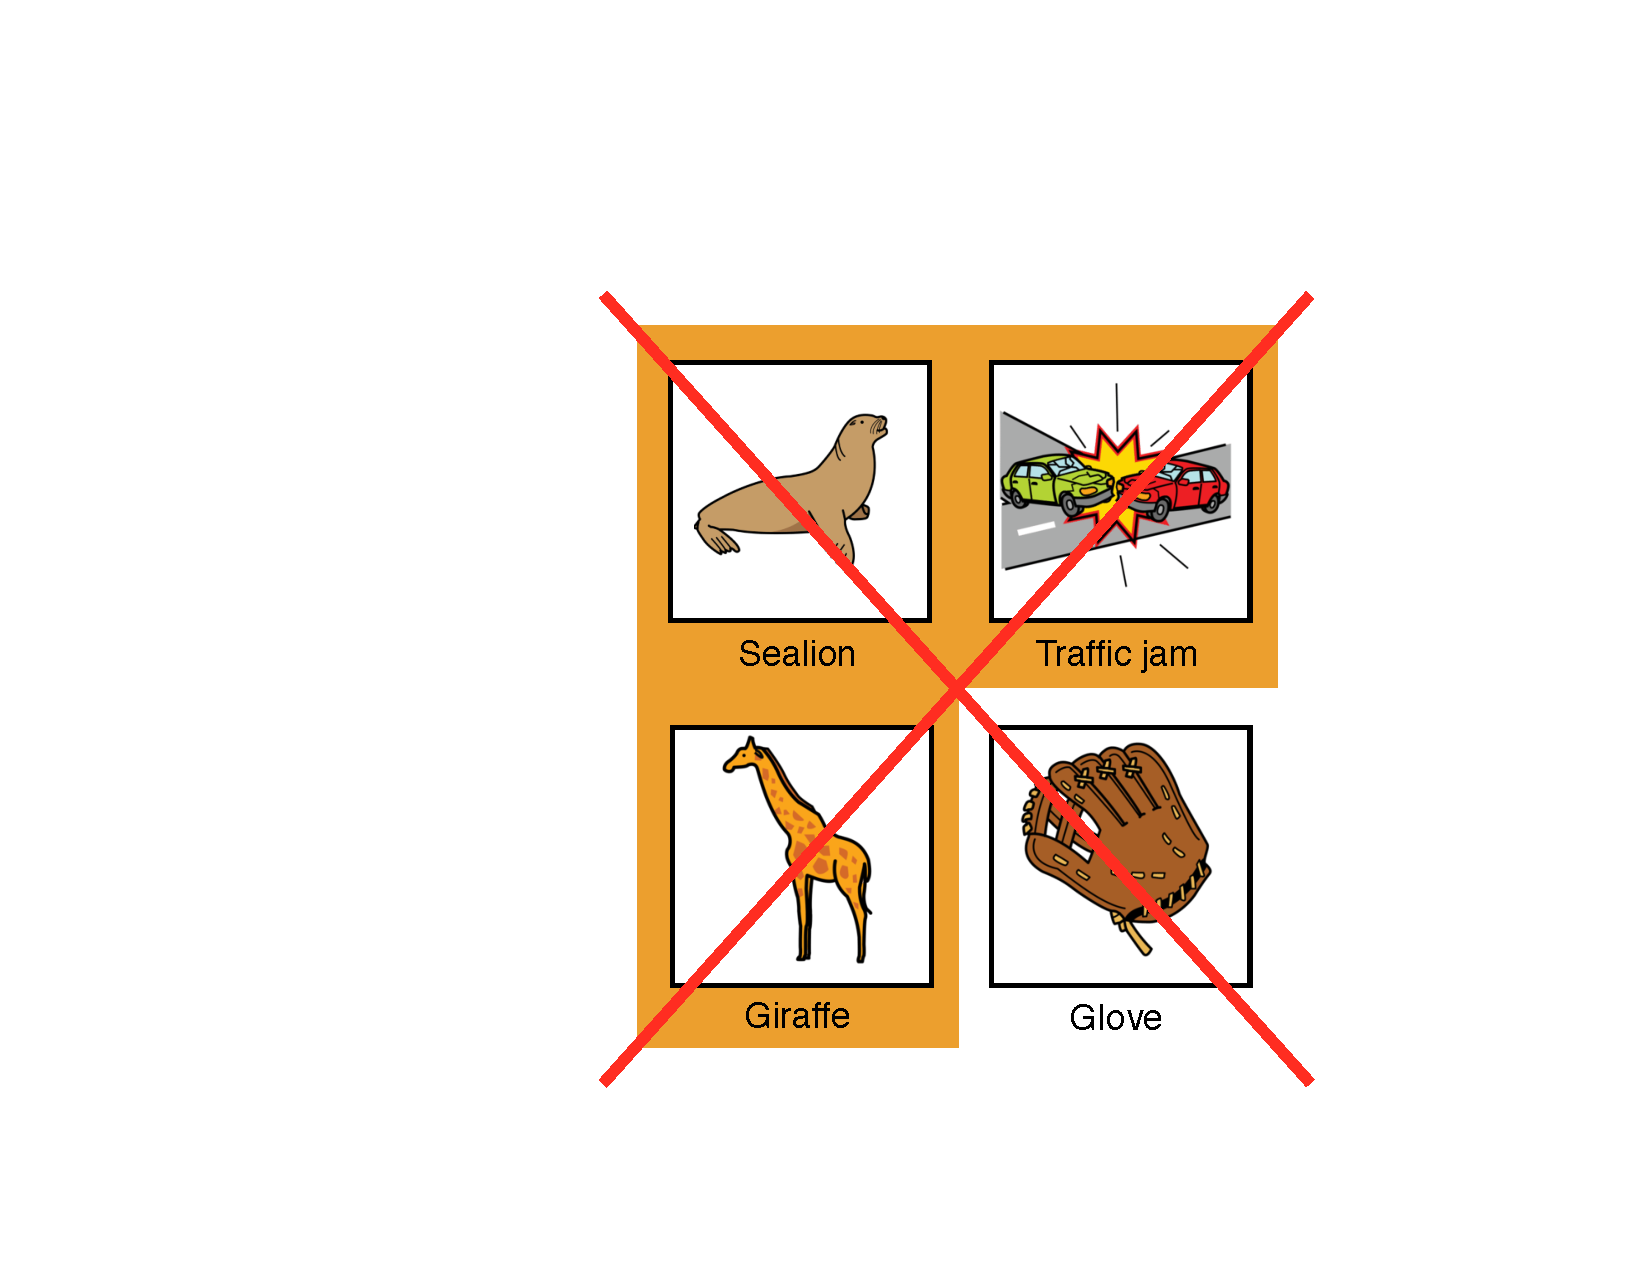
\includegraphics[scale=0.5]{pictograms_marked_wrong}
        \caption{Wrong marking}
        \label{fig:pictograms_marked_wrong}
    \end{subfigure}
    
    \caption{Marking of images}
    \label{fig:pictograms_marked}
\end{figure}

\begin{note}
	It is important that when having multiple marked images that there are some margin between these elements. And it should be implemted as seen on Figure \ref{fig:pictograms_marked_corect} not as seen on Figure \ref{fig:pictograms_marked_wrong}.
\end{note} 

\section{Indicator overlay}
\label{sec:indicator_overlay}

If one wants to indicate that an image is editable, for instance when picking an icon for a category, the image should have an overlay indicating this as seen on Figure \ref{fig:pictogram_indicator_overlay_editable}. Other types of indicator should look similar, like indicating that an image is the icon for a category is indicated as seen on \ref{fig:pictogram_indicator_overlay_category}.

\begin{figure}[!htbp]
    \centering

    \begin{subfigure}[t]{0.4\textwidth}
        \centering
        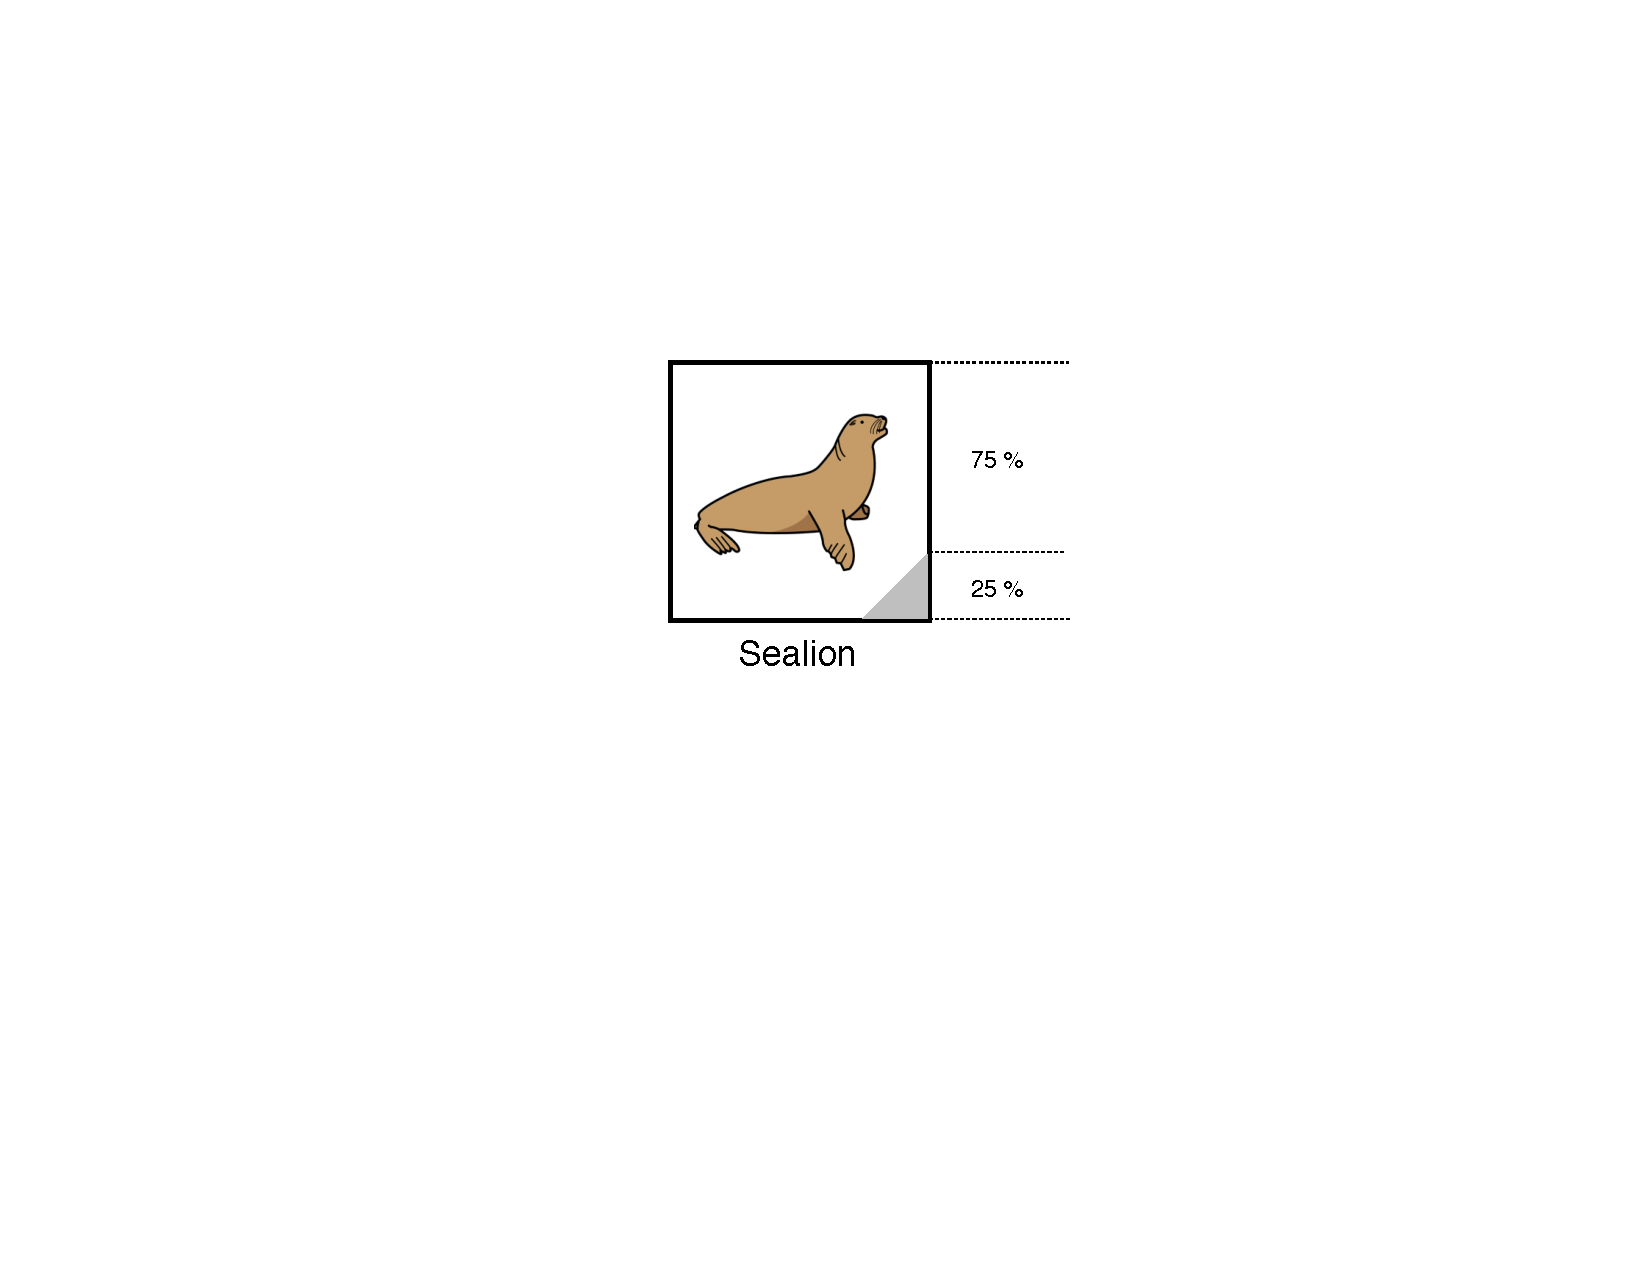
\includegraphics[scale=0.6]{pictogram_indicator_overlay_editable}
        \caption{Editable indicator}
        \label{fig:pictogram_indicator_overlay_editable}
    \end{subfigure}
    \hspace{5em} 
    \begin{subfigure}[t]{0.4\textwidth}
        \centering
        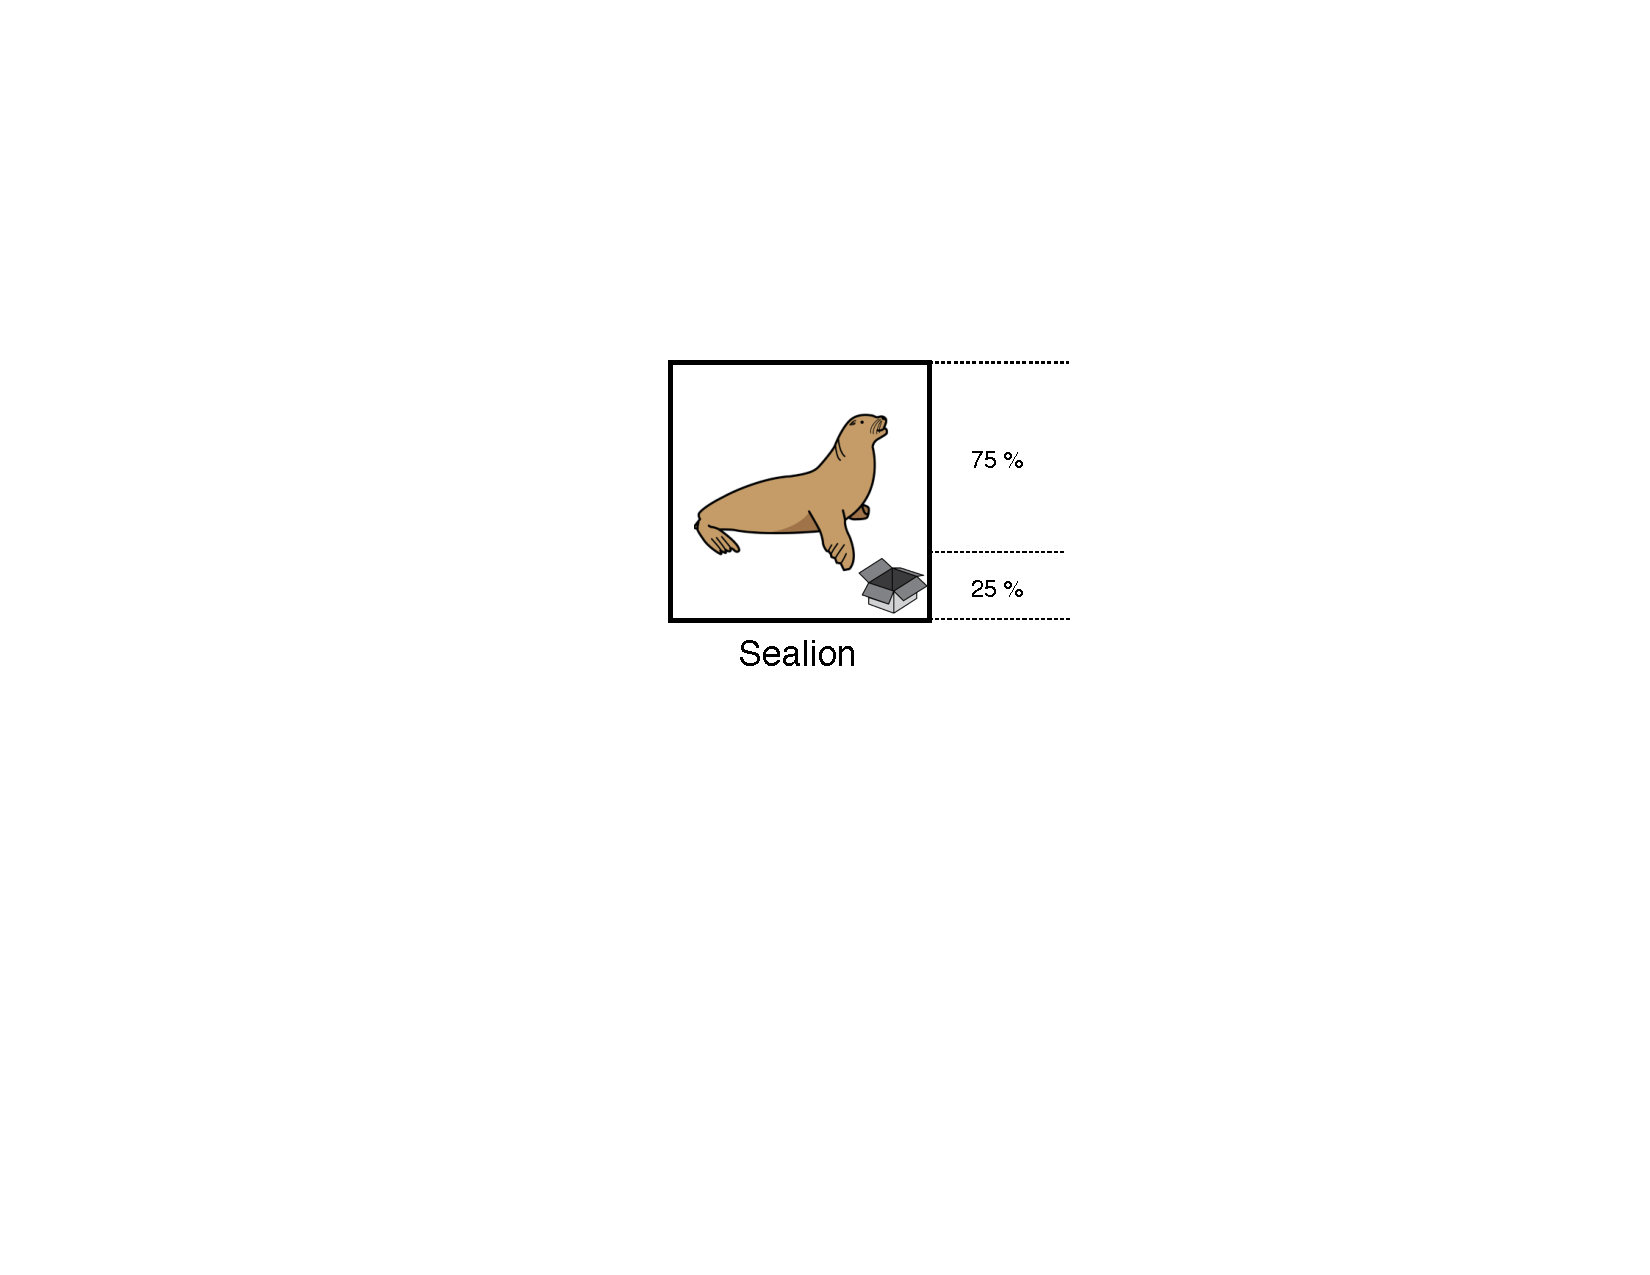
\includegraphics[scale=0.6]{pictogram_indicator_overlay_category}
        \caption{Category indicator}
        \label{fig:pictogram_indicator_overlay_category}
    \end{subfigure}
    
    \caption{Indicator overlays}
    \label{fig:pictograms_marked}
\end{figure}






























